% !TeX root = ../../thesis.tex
\chapter{This is datacuration}\label{ch:datacuration}

\ldots

In this chapter, I will describe how the dataset was created. I will discuss the reasons for the made choices in data seletection.


\section{Available data in Flanders}
Aerial imagery of Flanders is freely available. There are winter and summer images. The winter images are taken yearly in the spring. This has the advantage that foliage is not fully present yet. Summer imagery, however, has a NIR band on top of the RGB bands. This is useful in determining vegetation. The drawback, however, is that there are no pretrained CNNs available for extracting features from imagery with 4 bands. Therefore, I decided to limit the dataset to using spring imagery with three bands.

From previous research discussed in the previous chapter, w it was found that aerial imagery 


\section{Overview of the used data}

The used data layers are listed below. In each table the data layer is described.
\subsection{Base data}

\begin{itemize}
    \item Municipality boundaries
    \item Zoning plan "gewestplan"
    \item Aerial imagery
    \item Administrative boundaries
\end{itemize}

\subsubsection{Map of Flemish municipalities}
\begin{tabular}{l|l}
    \hline

    \multicolumn{2}{|c|}{
        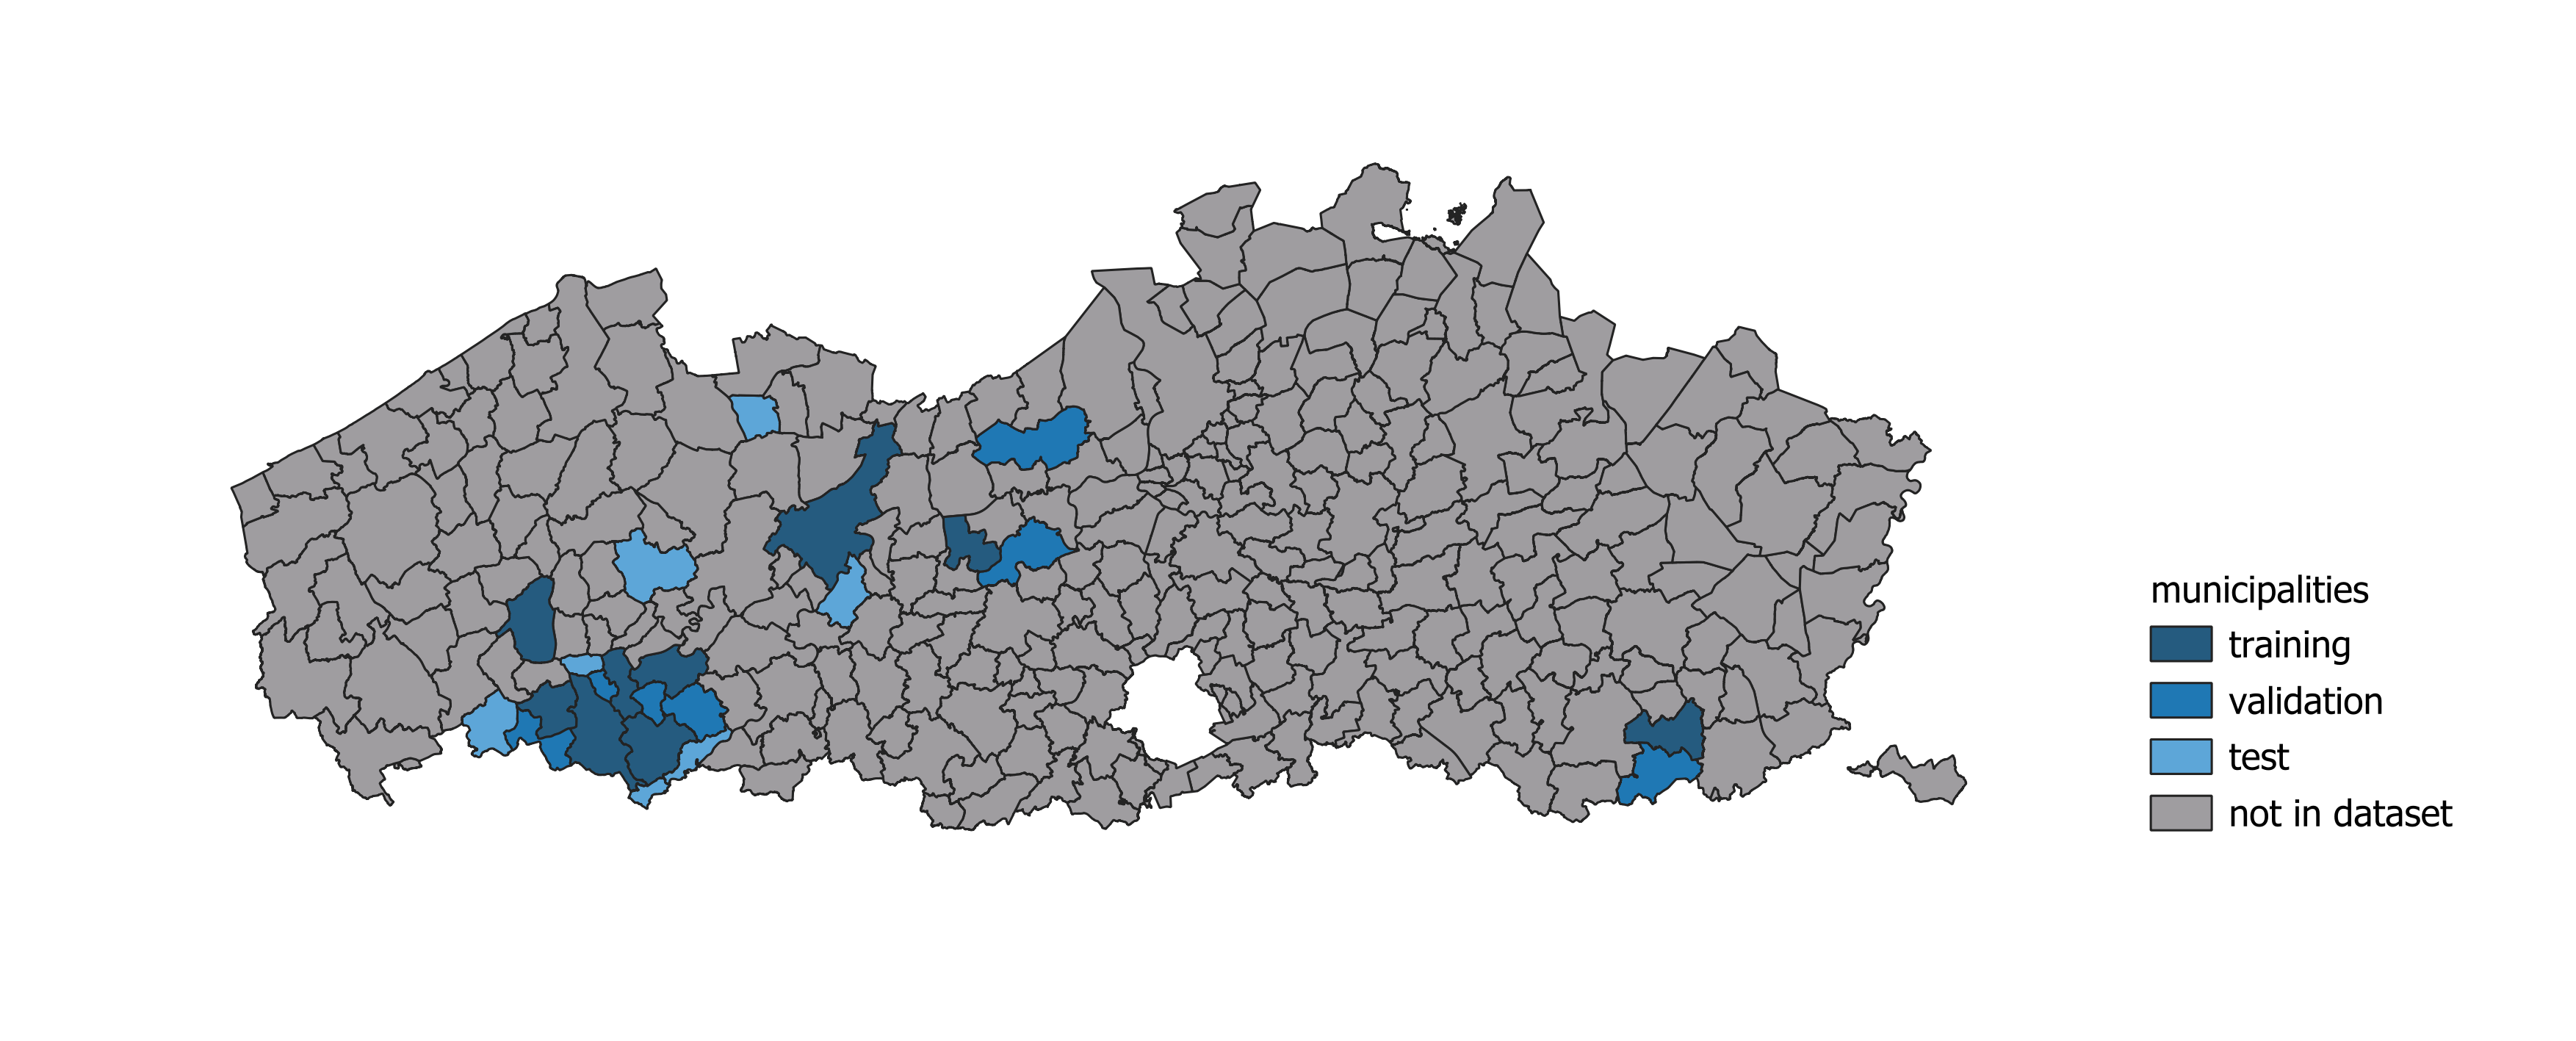
\includegraphics[width=0.8\linewidth]{image/Municipalities.png}
    } \\
    \hline
    \hline
    \textbf{Name Layer} & \textbf{Description} \\
    \hline
    \hline
    Shown data & The selected municipalities chosen for the creating of the dataset are shown on the map. The choices of municipalities were based on their representation across different regions of Flanders and data availability. \\
    \hline
    Data format & polygon shapefile \\
    \hline
    Data splits & gem_train = ['Kortrijk','Waregem', 'Wevelgem', 'Harelbeke','Zwevegem','Berlare','Gent','Roeselare','Borgloon']
    gem_val = ['Menen','Anzegem','Kuurne','Deerlijk','Dendermonde','Heers','Sint-Niklaas']
    gem_test = ['Avelgem','Lendelede','Wervik','Spiere-Helkijn','Eeklo','Merelbeke','Tielt']
\end{tabular}

\subsection{Zoning plan "gewestplan"}
\begin{tabular}{l|l}
    \hline
    \textbf{Original Name Layer} & \textbf{Description} \\
    \hline
    Shown data & descrition of the shown data \\
    \hline
    Data format & shapefile \\
    \hline
    Temporal resolution & yearly \\
    \hline
    Spectral resolution & RGB \\
    \hline
    Date & April, 2020 \- April 2021, ... \\
    \hline
    Source & Agentschap Informatie Vlaanderen \\
    \hline
    CRS & EPSG:31370 \\
    \hline
    Number of elements or size & NA \\
    \hline
\end{tabular}

\subsection{Aerial imagery}
\begin{tabular}{l|l}
    \hline
    \textbf{Original Name Layer} & \textbf{Description} \\
    \hline
    Shown data & descrition of the shown data \\
    \hline
    Data format & geotiff and jp2000 \\
    \hline
    Spatial resolution & 25cm \\
    \hline
    Temporal resolution & yearly \\
    \hline
    Spectral resolution & RGB \\
    \hline
    Date & April, 2020 \- April 2021, ... \\
    \hline
    Source & Agentschap Informatie Vlaanderen \\
    \hline
    CRS & EPSG:31370 \\
    \hline
    Number of elements or size & NA \\
    \hline
\end{tabular}

\subsection{Administrative boundaries}
\begin{tabular}{l|l}
    \hline
    \textbf{Original Name Layer} & \textbf{Description} \\
    \hline
    Shown data & descrition of the shown data \\
    \hline
    Data format & geotiff and jp2000 \\
    \hline
    Spatial resolution & 25cm \\
    \hline
    Temporal resolution & yearly \\
    \hline
    Spectral resolution & RGB \\
    \hline
    Date & April, 2020 \- April 2021, ... \\
    \hline
    Source & Agentschap Informatie Vlaanderen \\
    \hline
    CRS & EPSG:31370 \\
    \hline
    Number of elements or size & NA \\
    \hline
\end{tabular}


\subsection{Main data sources}
This section describes the main data sources which determined the use of the parcel.

\begin{itemize}
    \item VKBO
    \item Sports accomodations
    \item Agricultural parcels
    \item Points of Interest
    \item Company locations "Bedrijvengids"
\end{itemize}

\subsection{VKBO}
\begin{tabular}{l|l}
    \hline
    \textbf{Original Name Layer} & \textbf{Description} \\
    \hline
    Shown data & descrition of the shown data \\
    \hline
    Data format & geotiff and jp2000 \\
    \hline
    Spatial resolution & 25cm \\
    \hline
    Temporal resolution & yearly \\
    \hline
    Spectral resolution & RGB \\
    \hline
    Date &  \\
    \hline
    Source & Agentschap Informatie Vlaanderen \\
    \hline
    CRS & EPSG:31370 \\
    \hline
    Number of elements or size & NA \\
    \hline
\end{tabular}

\subsection{Sports accomodations}
\begin{tabular}{l|l}
    \includegraphics{}
    \hline
    \textbf{Original Name Layer} & \textbf{Description} \\
    \hline
    Shown data & Private dataset \\
    \hline
    Data format & point shapefile \\
    \hline
    Temporal resolution & yearly \\
    \hline
    Date & April, 2020 \- April 2021, ... \\
    \hline
    Source & Sport Vlaanderen \\
    \hline
    CRS & EPSG:31370 \\
    \hline
    Number of elements or size & NA \\
    \hline
\end{tabular}

\subsection{Agricultural parcels}
\begin{tabular}{l|l}
    \includegraphics{}
    \hline
    \textbf{Original Name Layer} & \textbf{Description} \\
    \hline
    Shown data & Private dataset \\
    \hline
    Data format & point shapefile \\
    \hline
    Temporal resolution & yearly \\
    \hline
    Date & April, 2020 \- April 2021, ... \\
    \hline
    Source & Sport Vlaanderen \\
    \hline
    CRS & EPSG:31370 \\
    \hline
    Number of elements or size & NA \\
    \hline
\end{tabular}

\subsection{Points of Interest}
\begin{tabular}{l|l}
    \includegraphics{}
    \hline
    \textbf{Original Name Layer} & \textbf{Description} \\
    \hline
    Shown data & Private dataset \\
    \hline
    Data format & WFS \\
    \hline
    Temporal resolution & yearly \\
    \hline
    Date & April, 2020 \- April 2021, ... \\
    \hline
    Source & Sport Vlaanderen \\
    \hline
    CRS & EPSG:31370 \\
    \hline
    Number of elements or size & NA \\
    \hline
\end{tabular}

\subsection{Data processing}

The data was processed for the purpose of creating small images suitable for training a convolutional neural network.
For the processing, pyQGIS was used on the linux server. Using HTCondor, large amounts of data could be processed in parallel.
The data was processed in the following way:
\begin{itemize}
    \item The main data source was loaded
    \item parcel data was loaded
    \item The zoning plan "gewestplan" was loaded
    \item The main data was filtered on location in the chosen municipalities
    \item The attribute of zoning area was added to each main data point
    \item The main data points were filtered on the relevant zoning areas
    \item The parcels containing the main data points were selected
    \item The attributes of the main data points were added to the selected parcels
    \item The raster was clipped using the selected parcels as extent
    \item The clipped raster was saved in RGB format with original dimensions
    \item The attributes and metadata was saved in an xml file
\end{itemize}



\subsection{Obtained dataset}

Here a summary and visualization of the obtained dataset is given. The dataset contains ... images of size ... with ... classes. The dataset is split into a training set, a validation set, and a test set. The training set contains ... images, the validation set contains ... images, and the test set contains ... images. The dataset is imbalanced, with ...\% of the images belonging to class 1, ...\% of the images belonging to class 2, and ...\% of the images belonging to class 3.

\subsubsection{Metadata storage}

In this section, the storage of the metadata is described. The metadata is stored in an xml file with attributes per image.
Below is an example of the metadata for one image. 

\subsection{Data Splits}

The dataset is split into training, validation, and test set based on the municipality. This was done to ensure that images of the same parcel taken over various years would always appear in the same split. The decision of which municipalities are in each split was done to ensure the best class balance.


\subsection{Shortcomings of the dataset}
\subsubsection{Class imbalance}

Show a graph of the class imbalance in the entire dataset and the subselection to reduce the class imbalance.


    %%%%%%%%%%%%%%%%%%%%%%%%%%%%%%%%%%%%%%%%%%%%%%%%%%
% Keep the following \cleardoublepage at the end of this file, 
% otherwise \includeonly includes empty pages.
\cleardoublepage

% vim: tw=70 nocindent expandtab foldmethod=marker foldmarker={{{}{,}{}}}
